\documentclass[11pt]{article}
\usepackage[utf8]{inputenc}
\usepackage[T1]{fontenc}
\usepackage{graphicx}
\usepackage{xcolor}
\usepackage{listings}
\usepackage{textcomp}
\usepackage[most]{tcolorbox}
\usepackage{pythonhighlight}
\usepackage{minted}
\usepackage{lscape}
\usepackage{rotating}
\usepackage{svg}
\usepackage[titletoc,title]{appendix}
\usepackage{animate}
\usepackage{subcaption}
%\usepackage{subfig;subfigure}
%\usepackage[dotinlabels]{titletoc}

%\usepackage[autostyle]{csquotes}

\usepackage[backend=bibtex,citestyle=authoryear,maxnames=1]{biblatex}
\addbibresource{biblio.bib}

\newcommand{\source}[1]{\vspace*{-0.4cm}\caption*{\textit{Source: {#1}}}}
\renewcommand{\contentsname}{Table des matières}
\newcommand{\mycite}[1]{ (\cite{#1})}
\newcommand{\tocheck}[1]{\textcolor{lightgrey}{#1}}
\newcommand{\tool}{\emph{FragScape}}
\newcommand{\qgis}{\emph{QGIS}}
\newcommand{\grass}{\emph{GRASS}}
\newcommand{\myfigureref}[1]{Figure \ref{#1} : \hyperref[#1]{\nameref{#1}}\dotfill\pageref{#1}}
\newcommand{\meff}{taille effective de maille}
\newcommand{\Meff}{TODO}



\lstset{upquote=true,
    language=Python,
    showspaces=false,
    basicstyle=\small\ttfamily,
    %numbers=left,
    %numberstyle=\tiny,
    commentstyle=\color{gray}
    xleftmargin=1cm,
    % Code design
    identifierstyle=\color{editorGray},
    keywordstyle=[1]\color{editorBlue}\bfseries,
    keywordstyle=[2]\color{editorBlue}\bfseries,
    keywordstyle=[3]\color{editorBlack}\bfseries,
    keywordstyle=[4]\color{editorBlue}\bfseries,
    commentstyle=\color{editorGray}\ttfamily,
    stringstyle=\color{editorGreen}}

\definecolor{FunctionName}{rgb}{0,150,0}

% 2079971ms

\definecolor{editorLightGray}{cmyk}{0.05, 0.05, 0.05, 0.1}
\definecolor{editorWhite}{cmyk}{0, 0, 0, 0}
\definecolor{editorOrange}{cmyk}{0, 0.8, 1, 0}
\definecolor{editorBlue}{cmyk}{1, 0.6, 0, 0}
\definecolor{editorGreen}{rgb}{0, 0.5, 0}
\definecolor{editorGray}{black}{0.9}

\input{defs}

\usepackage{lipsum}
\usepackage{arydshln}
\usepackage{hyperref}

\usepackage{biblatex}
\addbibresource{biblio.bib}

\usepackage{fancyhdr}
\usepackage{lastpage}

\usepackage{indentfirst}

\pagestyle{fancy}
\fancyhf{}

\setlength{\headsep}{1.3in}
\setlength{\voffset}{-30pt}
\setlength\parindent{0pt}


\let\tempone\itemize
\let\temptwo\enditemize
\renewenvironment{itemize}{\tempone\addtolength{\itemsep}{-0.5\baselineskip}}{\temptwo}
\renewenvironment{enumerate}{\tempone\addtolength{\itemsep}{-0.5\baselineskip}}{\temptwo}


%%%%%%%%%%%%%%%
% Title Page
\bigskip
%\title{Développement d'un plugin \emph{QGIS} pour modéliser les déplacements de la faune par la méthode de perméabilité des milieux pour la cartographie des continuités écologiques}
%\title{Titre quand meme plus court sinon c'est relou}
\bigskip

\date{\today}
%\summary{}
%%%%%%%%%%%%%%%

\begin{document}

\renewcommand{\appendixtocname}{Annexes}
\renewcommand{\appendixpagename}{\color{color1}{Annexes}} 
\sloppy

%\pagestyle{style2}

\vspace{4cm}

\maketitle

\clearpage

\pagestyle{style1}

\setlength{\headsep}{0.9in}

\tableofcontents

\hspace{4cm}

%\section*{Table des figures}


%\myfigureref{biogeoFragm}


%\pagebreak

%\section*{Table des figures}

\pagebreak

\section{Aperçu}

\tool\ est un plugin \qgis\ permettant de calculer les indicateurs de fragmentation du paysage définis dans l'article « Landscape division, splitting index, and effective mesh size: new measures of landscape fragmentation » \mycite{jaeger}.
Parmi ces indicateurs, la taille effective de maille est très largement utilisée pour quantifier la fragmentation du paysage. \tool\ définit une procédure en 4 étapes depuis les données brutes jusqu'au calcul des indicateurs et permet de sauvegarder la configuration de l'outil afin de pouvoir reproduire les résultats.

\subsection{Indicateurs de fragmentation du paysage}
\label{sec:metrics}

Jaeger définit dans son article\mycite{jaeger} trois nouvelles mesures de fragmentation du paysage :
\begin{itemize}
    \item le degré de fragmentation du paysage 
    \item le nombre effectif de mailles
    \item la taille effective de maille
\end{itemize}

Pour calculer ces indicateurs, les éléments du paysage considérés comme fragmentants sont retirés. Les éléments restants sont appelés « patchs ». Le paysage est alors composé de $n$ patchs. La superficie d'un patch est notée  $A_i$ avec $1 \leq i \leq n$. La superficie totale du territoire d'étude est notée $A_t$.

\subsubsection{Degré de fragmentation du paysage}

Le degré de cohérence ($C$ ou $COH$), une mesure auxiliaire, est défini comme la probabilité que deux points choisis aléatoirement dans le territoire soient connectés (c.à.d. non séparés par des éléments fragmentants comme des routes ou des zones urbaines).

Le degré de fragmentation du paysage ($D$ ou $DIVI$) est défini comme la probabilité que deux points choisis aléatoirement dans le territoire ne soient $pas$ connectés.

\hspace*{-0.5cm}
\begin{minipage}[c][1cm]{.46\linewidth}
\begin{align*}
C = \sum_{i=1}^{n}(\frac{A_{i}}{A_{t}})^{²}
\end{align*}
\end{minipage}
\begin{minipage}[c][1cm]{.46\linewidth}
\begin{align*}
D = 1 - C
\end{align*}
\end{minipage}

\subsubsection{Nombre effectif de mailles}

Le nombre effectif de mailles ($S$ ou $SPLI$) est défini comme le nombre de patchs obtenu en découpant la superficie totale du territoire par une maille régulière de telle façon que la nouvelle configuration mène au même degré de fragmentation que la configuration initiale :
\begin{align*}
S = \frac{A_{t}^{2}}{\sum_{i=1}^{n}A_{i}^{2}}
\end{align*}

$S$ peut être interprété comme le nombre effectif de maille effectif d'un réseau avec une taille de maille constante divisant le territoire en $S$ patchs de taille $A_{t} / S$.

\subsubsection{Taille effective de maille}

La taille effective de maille ($m$ ou $MSIZ$) correspond à la taille des patchs quand le territoire est divisé en $S$ patchs (chacun de même taille $At/S$) avec le même degré de fragmentation que la configuration initiale :
\begin{align*}
m = \frac{A_{t}}{S} = \frac{1}{A_{t}}\sum_{i=1}^{n}A_{i}^{2}
\end{align*}

La densité de mailles ($s$ ou $SDEN$) correspond au nombre de mailles par unité de surface.
Le produit net ($N$ ou $NPRO$) est défini comme le produit de la taille effective de maille $m$ par la superficie totale du territoire.

\hspace*{-0.5cm}
\begin{minipage}[c][1cm]{.46\linewidth}
\begin{align*}
s = \frac{S}{A_{t}} = \frac{A_{t}}{\sum_{i=1}^{n}A_{i}^{2}} = \frac{1}{m}
\end{align*}
\end{minipage}
\begin{minipage}[c][1cm]{.46\linewidth}
\begin{align*}
N = m.{A_{t}} = \sum_{i=1}^{n}A_{i}^{2}
\end{align*}
\end{minipage}

%$S = \frac{S}{A_{t}} = \frac{A_{t}}{\sum_{i=1}^{n}A_{i}^{2}} = \frac{A_{t}}{S}$

%Le produit net ($N$) est défini comme le prorduit de la taille effective de maille $m$ par la superficie totale du territoire : $\frac{1}{A_{t}}\sum_{i=1}^{n}A_{i}^{2}$



\subsubsection{Méthode « Cross-Boundary Connections » (CBC)}
\label{sec:cbc}

Comme d'autres indicateurs du paysage basés sur la notion de patch, les indicateurs définis ci-dessus peuvent être biaisés car les limites du territoire sont considérées comme fragmentantes et peuvent ainsi artificiellement découper les patchs. Pour répondre à ce problème, l'article « Modification of the effective mesh size for measuring landscape fragmentation to solve the boundary problem »\mycite{moser} propose une nouvelle méthode de calcul.

Cette méthode, appelée \textit{Cross-Boundary Connections} (CBC), inclut la superficie des patchs à l'extérieur des « frontières » du territoire. La superficie totale d'un patch est notée $A_{i}^{cmpl}$. La somme de la superficie des patchs est notée $A_{total}^{cmpl}$. La formule de la taille effective de maille d'après la méthode CBC ($m_{CBC}$ ou $CBC\_MSIZ$) est alors :
\hspace*{-2.5cm}
\begin{align*}
m_{CBC} = \frac{1}{A_{t}}\sum_{i=1}^{n}A_{i}.A_{i}^{cmpl}
\end{align*}

\hspace*{-2.5cm}
\frameboxbegin{Métriques CBC}
\textbf{\color{red}En mode CBC, seules 2 métriques sont définies : la taille effective de maille et le produit net}
\frameboxend

%Les autres indicateurs sont adaptés à la méthode CBC, ainsi les expressions $\sum_{i=1}^{n}A_{i}^{2}$ et $A_{t}^{2}$ sont respectivement remplacéees par les expressions $\sum_{i=1}^{n}A_{i}.A_{i}^{cmpl}$ et $A_{t}.A_{total}^{cmpl}$.

\subsection{Méthodes de calcul}
\label{sec:mode}

Le calcul des indicateurs se base sur une couche contenant les patchs d'espaces naturels.

\tool\ permet d'accompagner l'utilisateur dans la constitution de cette couche de patchs en plusieurs étapes (détails en section \ref{sec:steps}) depuis les données d'entrées brutes (occupation du sol, routes, ...). Il permet de sélectionner les éléments naturels et semi-naturels de l'occupation du sol puis de leur intégrer les données complémentaires.

Il existe 2 modes de calcul en fonction du type des données d'entrée, de leur étendue, du besoin de précision et des ressources informatiques. Si la couche d'occupation du sol est au format Vecteur et que le volume de données est raisonnable (cf section \ref{sec:execTime}), le mode Vecteur est approprié. Si la couche d'occupation du sol est au format Raster ou que les données sont trop lourdes à traiter (large étendue spatiale, haute précision géométrique, ...), le mode Raster est approprié.

\subsubsection{Mode vecteur}

En mode vecteur, les entités sont sélectionnées depuis la couche d'occupation du sol et leur géométrie est agrégée (une seule entité de type MultiPolygon).

Il est alors possible d'ajouter des données complémentaires (au format vecteur) comme le réseau routier, le réseau hydrographique, ou encore toute donnée qui serait manquante dans la couche initiale. Ces données peuvent être affinées en effectuant une sélection (routes goudronnées par exemple) et en appliquant une zone tampon pour modéliser leur empreinte en sol en cas d'entités linéaires.

Toutes ces données sont alors intégrées à l'occupation du sol, par union si elles représentent des milieux naturels ou semi-naturels, et par différence si elles participent à la fragmentation du territoire. La couche résultante de ces opérations est agrégée (par géométrie) puis convertie en géométrie simple (Polygon) afin de construire une couche de patchs correcte pour le calcul des indicateurs.

\subsubsection{Mode raster}

En mode raster, les données sources peuvent être au format vecteur ou raster mais les couche produites seront au format raster dans tous les cas (rastérisation et reprojection selon les paramètres d'emprise et de résolution définis).

Le choix de la résolution est primordial car il définit la précision des données mais aussi la mémoire vive nécessaire (cf section \ref{sec:execTime}). Si l'occupation du sol est déjà au format raster, il est conseillé de garder la même résolution.

La couche d'occupation du sol est reclassifiée : 1 pour les éléments naturels (classes sélectionnées), 0 pour les éléments de fragmentation (classes non sélectionnées).
Les données complémentaires sont reprojetées et classifiées de la même façon. Les couches résultantes sont alors fusionnées selon l'ordre spécifié dans l'interface graphique.


\subsection{Installation}

\tool\ est un plugin \qgis. \tool\ a été testé sur différents systèmes d'exploitation : Ubuntu bionic, Windows 10 et macOS Sierra.

\frameboxbegin{Prérequis}
\begin{itemize}
    \item \textbf{\color{red}La version de \qgis\ doit être supérieure ou égale à 3.4.0.}
    \item \textbf{\color{red}Les bibliothèques python \emph{scipy} et \emph{numpy} doivent être déjà installées pour utiliser le mode raster (cf section \ref{sec:err}).}
\end{itemize}
\frameboxend

Pour installer \tool, ouvrir \qgis:
\begin{enumerate}
    \item aller dans le menu \texttt{Extension}
    \item ouvrir la fenêtre \texttt{Installer/Gérer les extensions}
    \item aller dans l'onglet \texttt{Paramètres} et vérifier que l'option \texttt{Montrer les extensions expérimentales} est cochée
    \item retourner dans l'onglet \texttt{Toutes}, taper \tool\ dans la barre de recherche, sélectionner le résultat et appuyer sur le bouton \texttt{Installer le plugin}
\end{enumerate}

Une fois installé, l'icône \includesvg{pictures/vector_grid.svg} de \tool\ devrait appraître dans la barre d'outils de QGIS.

Si ce n'est pas le cas, aller dans le menu \texttt{Extension} et une entrée \tool\ devrait être présente.

Si ce n'est toujours pas le cas, l'installation a échoué. Vérifier les messages d'erreur ou contacter l'équipe de support.

\subsection{Interface graphique}

La figure \ref{fig:paramsTab} montre un aperçu de l'interface de \tool. Elle est composée de 4 prinicpaux éléments :
\begin{itemize}
    \item la barre d'outils en haut : chargement/enregistrement de la configuration, changement de langue 
    \item le panneau d'aide à droite : description de l'étape courante
    \item la barre de progression en bas : avancée du traitement en cours
    \item le fenêtre principale : contenu de l'étape courante
\end{itemize}

\begin{figure}[h!]
    \centering
    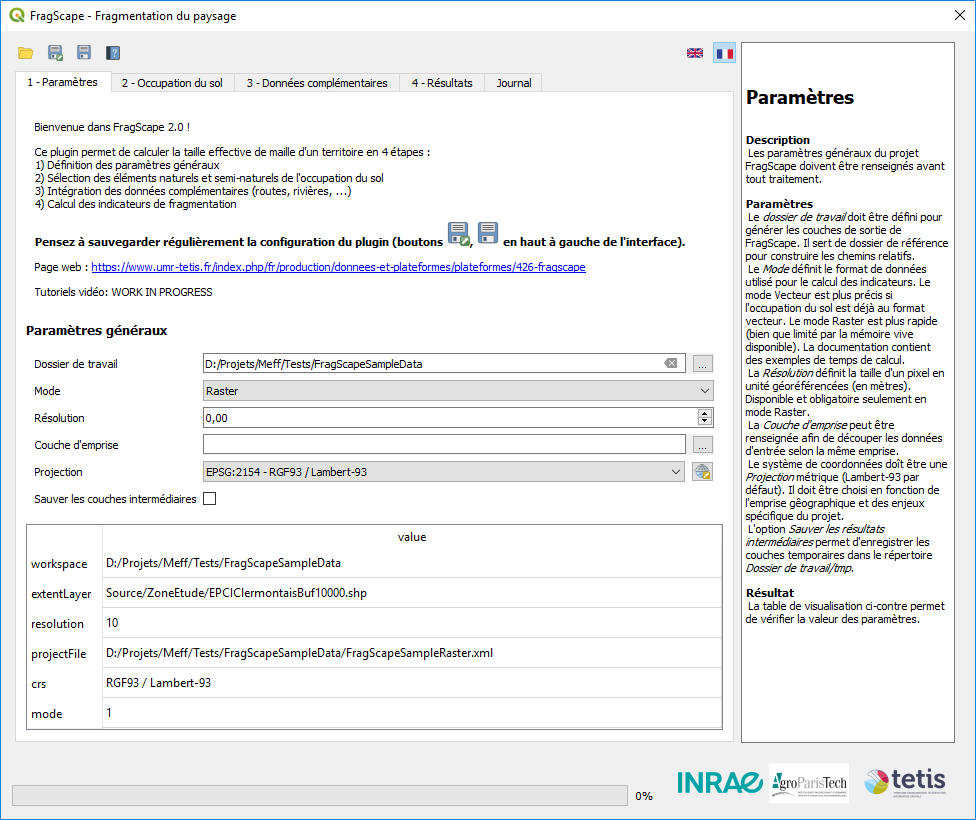
\includegraphics[scale=0.68]{pictures/paramsTabFr_v2.png}
    \caption{Interface graphique de \tool\ v2.0}
    \label{fig:paramsTab}
    %\source{\tool\ v1.0}
\end{figure}

Dans la fenêtre principale, l'étape courante peut être composée de :
\begin{itemize}
    \item paramètres à renseigner (\texttt{Dossier de travail} par exemple)
    \item une table de visualisation permettant de vérifier la valeur actuelle des paramètres
    \item des boutons d'action (\texttt{Lancer la sélection} par exemple)
\end{itemize}

\pagebreak

\section{Étapes}
\label{sec:steps}

\tool\ définit une procédure en 4 étapes depuis les données brutes jusqu'au calcul des indicateurs.

\subsection{Paramètres}

La première étape est de définir les paramètres globaux du projet \tool\ courant.

Le \texttt{Dossier de travail} doit être renseigné avant tout traitement car il définit le répertoire de sortie de \tool. Le résultat de chaque étape est stocké dans \textit{DossierDeTravail/outputs}. Attention au choix du dossier de travail car les fichiers déjà produits par \tool\ dans ce répertoire seront effacés.

Le \texttt{Mode} détermine la chaîne de traitements à exécuter pour le calcul des indicateurs (cf section \ref{sec:mode}). En mode Raster, il faut préciser une \texttt{Résolution} qui correspond à la taille d'un pixel en unités géoréférencées (mètre pour une projection métrique).

La \texttt{Couche d'emprise} définit l'emprise des données (elles sont découpées aux limites de la couche). Optionnel en mode vecteur. Pour le mode CBC, les données doivent s'étendre au-delà du territoire étudié.

La \texttt{Projection} est un système de projection cartographique qui doit être \textbf{métrique} et choisi en fonction de l'emprise des données. Il définit notammenet la forme et la superficie des entités.

%Si l'option \texttt{Sauver les couches intermédiaires} est cochée, les couches intermédiaires sont enregistrées dans le répertoire \textit{DossierDeTravail/tmp}. Sinon, elles sont stockées dans le répertoire de traitements temporaire \qgis\ (le chemin est indiqué lors de sa création dans le journal).

%\pagebreak

\subsection{Occupation du sol}

La deuxième étape est de sélectionner les éléments de l'occupation du sol considérés comme non-fragmentants (milieux naturels et semi-naturels). Pour ce faire il faut :
\begin{enumerate}
    \item Sélectionner la couche d'occupation du sol (paramètre \texttt{Couche d'entrée}).
    \item Choisir le \texttt{Mode} et le \texttt{Champ de sélection} si c'est une couche vecteur
    \item \texttt{Afficher les valeurs de champ} en appuyant sur le bouton 
    \item Cocher les postes d'occupation du sols correspondants aux milieux naturels dans la colonne \texttt{toSelect} de la table.
    \item Appuyer sur le bouton \texttt{Lancer la sélection}. La couche résultante chargée dans \qgis\ est produite dans le répertoire $DossierDeTravail/outputs$ ($landuseSelectionDissolve.gpkg$ en mode vecteur, $landuseSelectionWarp.tif$ en mode raster).
\end{enumerate}

\vspace*{-0.5cm}
\frameboxbegin{Mode de sélection}
En mode \texttt{Vecteur}, il existe deux modes de sélection :
\vspace*{-0.2cm}
\begin{itemize}
\item \texttt{Par valeur de champ} pour extraire les valeurs uniques du \texttt{Champ de sélection}
\item \texttt{Par expression} pour extraire les entités vérifiant l'expression renseignée (toutes les entités si l'expression est vide)
\end{itemize}
\vspace*{-0.2cm}
En mode \texttt{Raster}, les valeurs uniques de la première bande sont extraites.
\frameboxend

La figure \ref{fig:landuseTab} montre un exemple d'utilisation de l'interface de sélection de l'occupation du sol.

\begin{figure}[h!]
    \centering
    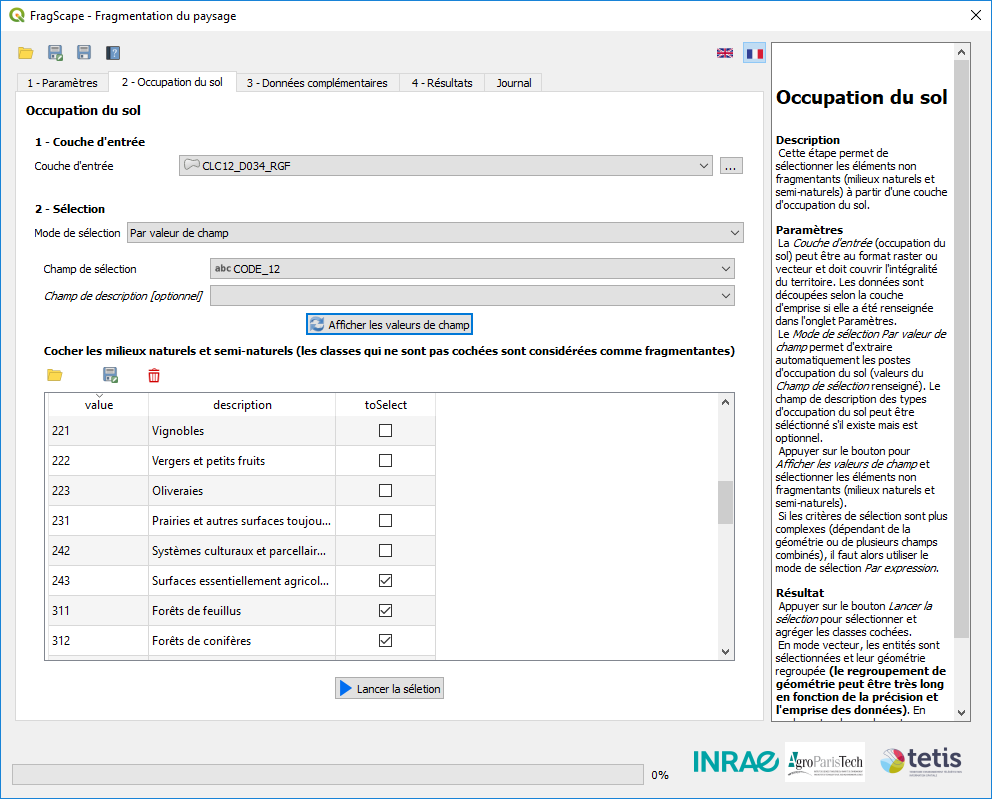
\includegraphics[scale=0.6]{pictures/landuseTabFr_v2.png}
    \caption{Onglet \textit{Occupation du sol} de \tool\ v2.0}
    \label{fig:landuseTab}
    %\source{\tool\ v1.0}
\end{figure}

\subsection{Données complémentaires}

La troisième étape permet d'intégrer des données complémentaires qui seraient manquantes ou pas assez précises dans l'occupation du sol. Par exemple : les routes, les cours d'eau, les passages à faune, etc.

Pour chaque source de données, il faut:
\begin{enumerate}
    \item Sélectionner la \texttt{Couche d'entrée} qui contient ces données
    %\item Si besoin, sélectionner l'option \texttt{Couper les données d'entrée} et choisir une \texttt{Couche de découpage}.
    \item (optionnel) Filtrer les entités en fonction d'une \texttt{Expression} (toute la couche est sélectionnée si l'expression est vide). L'expression peut être construite depuis le widget \includesvg{pictures/mIconExpression.svg}.
    \item Pour les entités ponctuelles et linéaires, définir une zone \texttt{Tampon} pour modéliser l'emprise au sol. L'expression (numérique) peut être variable et construite depuis le widget \includesvg{pictures/mIconExpression.svg}.
    \item Renseigner un \texttt{Identifiant} (unique dans le projet) pour cette sélection de données.
    \item Spécifier si ces données contribuent à la \texttt{Fragmentation} ou non
    \item Appuyer sur le bouton \texttt{Enregistrer la sélection}. La sélection renseignée apparaît alors comme un nouvelle ligne dans la table de visualisation.
\end{enumerate}

Une fois tous les données sélectionnées, il faut les \textbf{hiérarchiser} selon leur priorité (par exemple les passages à faune au-dessus des routes) puis appuyer sur le bouton \texttt{Intégrer les données complémentaires}.

Pour chaque ligne, les données sont sélectionnées, la zone tampon (si elle est définie) est appliquée et la couche est rastérisée pour le mode raster. Les couches ainsi obtenues sont alors fusionnées et le résultat de cette fusion est intégré au résultat de l'étape précédente. 
%pour calculer la différence avec la couche d'occupation du sol (l'intersection est supprimée). Enfin, cette différence est convertie en géométrie simple.

La couche finale est chargée dans QGIS et sauvegardée dans le dossier de sortie ( $landuseFragmSingleGeom.gpkg$ en mode vecteur, $landuseFragm.tif$ en mode raster).

\begin{figure}[h!]
    \centering
    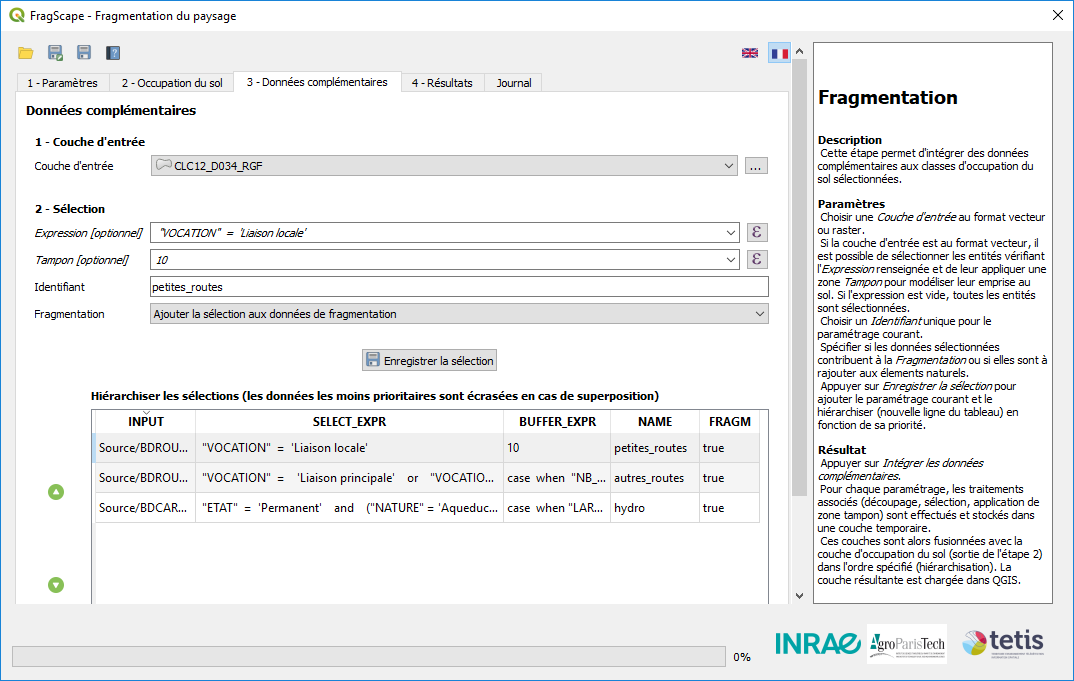
\includegraphics[scale=0.6]{pictures/fragmTabFr_v2.png}
    \caption{Onglet \textit{Données complémentaires} de \tool\ v2.0}
    \label{fig:fragmTab}
    %\source{\tool\ v1.0}
\end{figure}

\subsection{Résultats}

La quatrième étape est le calcul des indicateurs de fragmentation. Pour ce faire:
\begin{itemize}
    \item Spécifier la  \texttt{Couche d'entrée} (résultat de l'étape 3 par défaut).
    \item Renseigner la \texttt{Couche de rapportage}. Les indicateurs sont calculés pour chaque unité de rapportage. Pour calculer les indicateurs sur l'ensemble du territoire, la couche de rapportage doit ne contenir qu'une seule entité.
    \item Cocher l'option \texttt{Include les métriques CBC} si nécessaire (cf section \ref{sec:cbc})
    \item Sélectionner l'\texttt{Unité de surface} (du mètre carré au kilomètre carré).
    \item Renseigner la \texttt{Couche de sortie}. Si la couche n'est pas reseignée, une couche mémoire est créée.
    \item Appuyer sur le bouton \texttt{Calculer les idicateurs}.
\end{itemize}

\begin{figure}[h!]
    \centering
    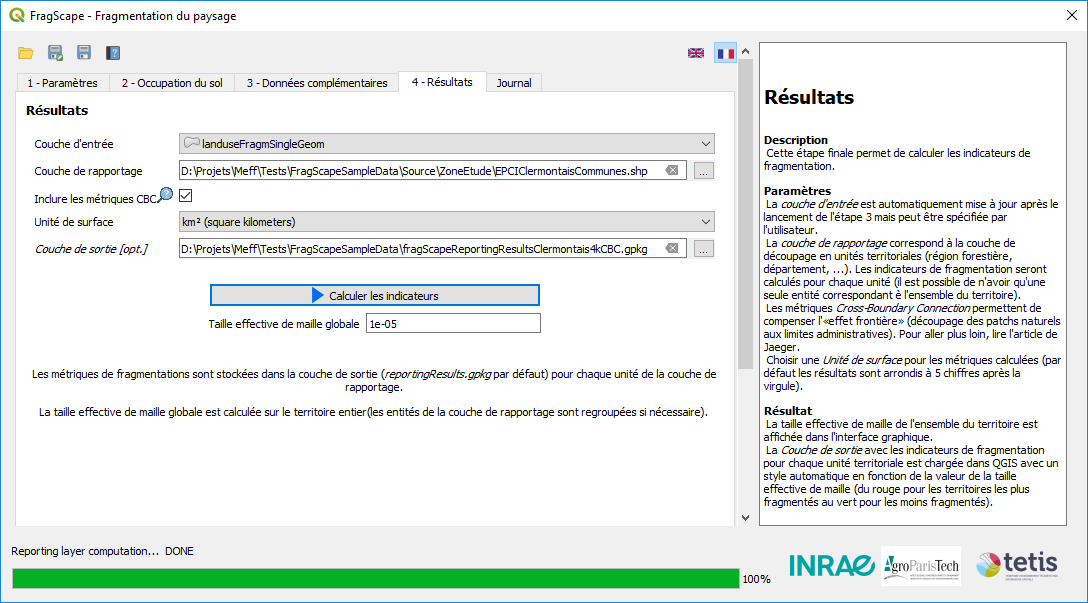
\includegraphics[scale=0.6]{pictures/resTabFr_v2.png}
    \caption{Onglet \textit{Résultats} de \tool\ v2.0}
    \label{fig:resultsTab}
    %\source{\tool\ v1.0}
\end{figure}


La figure \ref{fig:resultsTab} montre l'interface de cette dernière étape.
Une fois les indicateurs calculés, la couche de sortie est chargée dans QGIS et la taille effective de maille globale (sur l'ensemble du territoire) est affichée.
La couche de sortie contient un champ pour chaque métrique définie en section \ref{sec:metrics} plus de nouveaux champs :
\begin{itemize}
    \item \texttt{patches} : le nombre de patchs intersectant l'unité de rapportage
    \item \texttt{At} : l'aire de l'unité de rapportage
    \item \texttt{sum\_Ai} : l'aire de l'intersection entre les patchs et l'unité de rapportage
    \item \texttt{layer/path} : couche temporaire contenant l'unité de rapportage initiale
    \item \texttt{divisor} : diviseur correspondant à l'unité de surface (100 pour des décamètres carrés par exemple)
\end{itemize}

\pagebreaks

\section{Exemple}

Cette section montre un cas d'utilisation de \tool\ basé sur les données d'exemple (fournies avec le plugin dans le répertoire \href{https://github.com/MathieuChailloux/FragScape/tree/master/sample_data/EPCI_Clermontais_2012}{\texttt{sample\_data}}).

\begin{figure}[h!]
\centering
   \begin{subfigure}[b]{.48\textwidth}
      \includegraphics[width=\textwidth]{pictures/landuseInput.png}
      %\includegraphics[width=\textwidth]{pictures/CBC/landuseInput.png}
      \caption{Occupation du sol initiale}
   \end{subfigure}
   \begin{subfigure}[b]{.48\textwidth}
      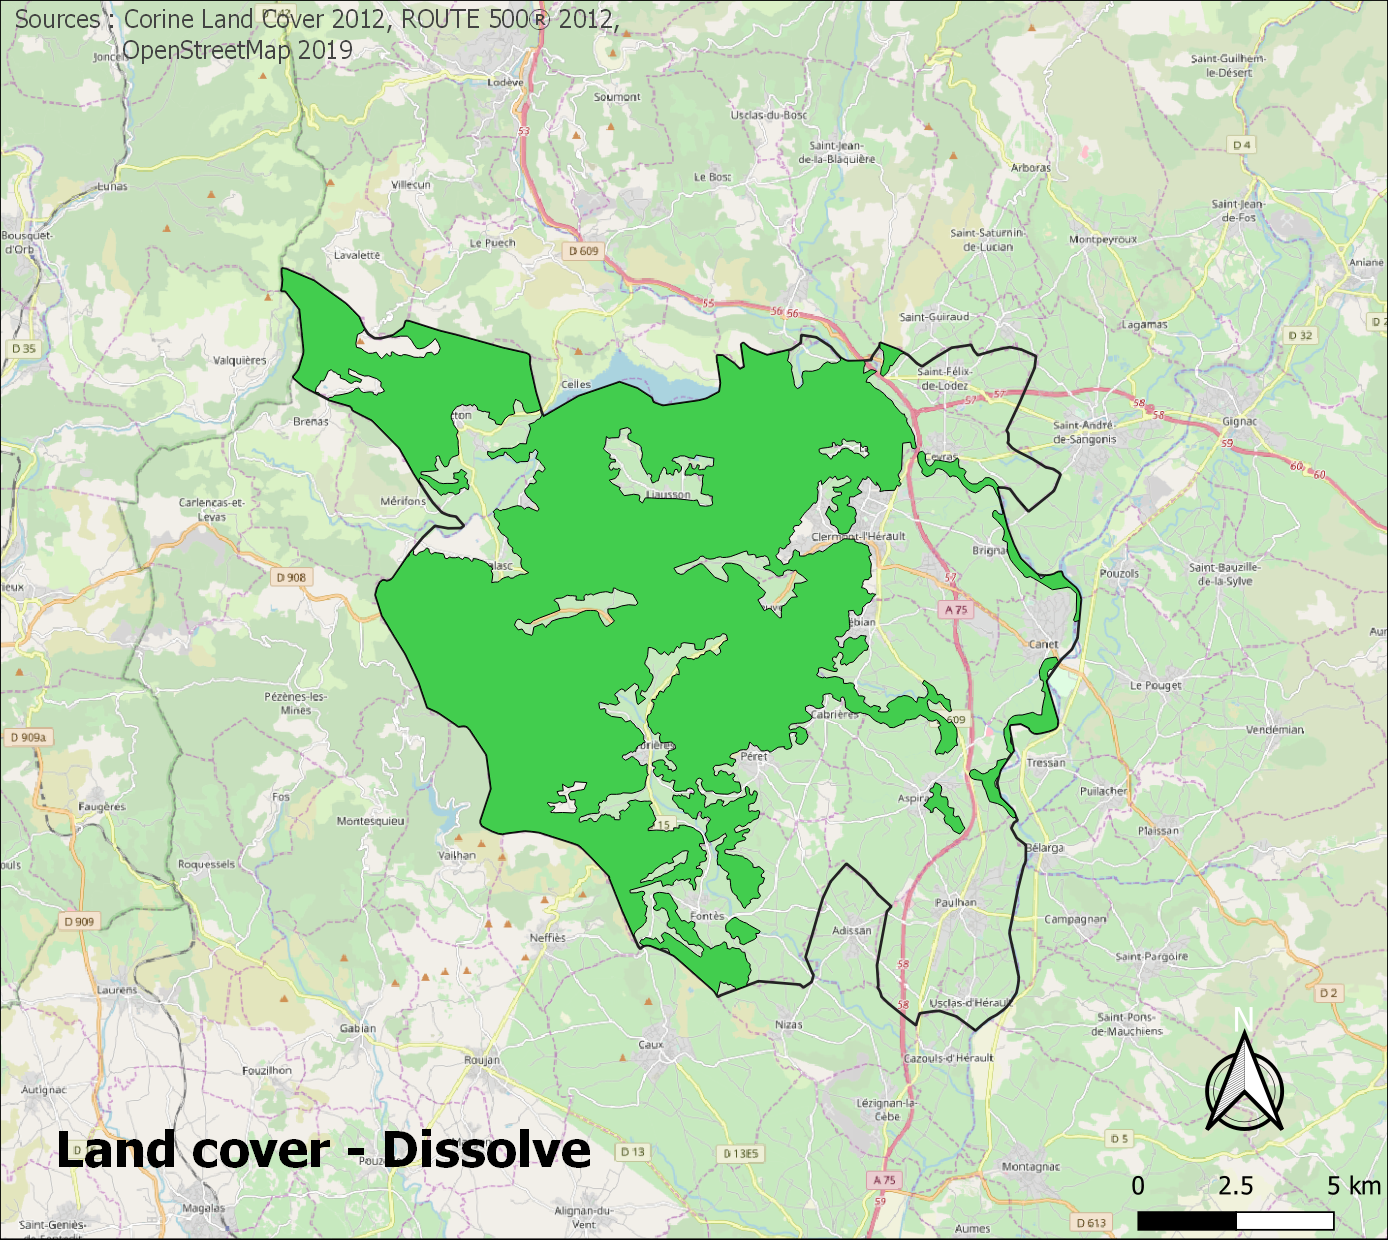
\includegraphics[width=\textwidth]{pictures/landuseDissolve.png}
      %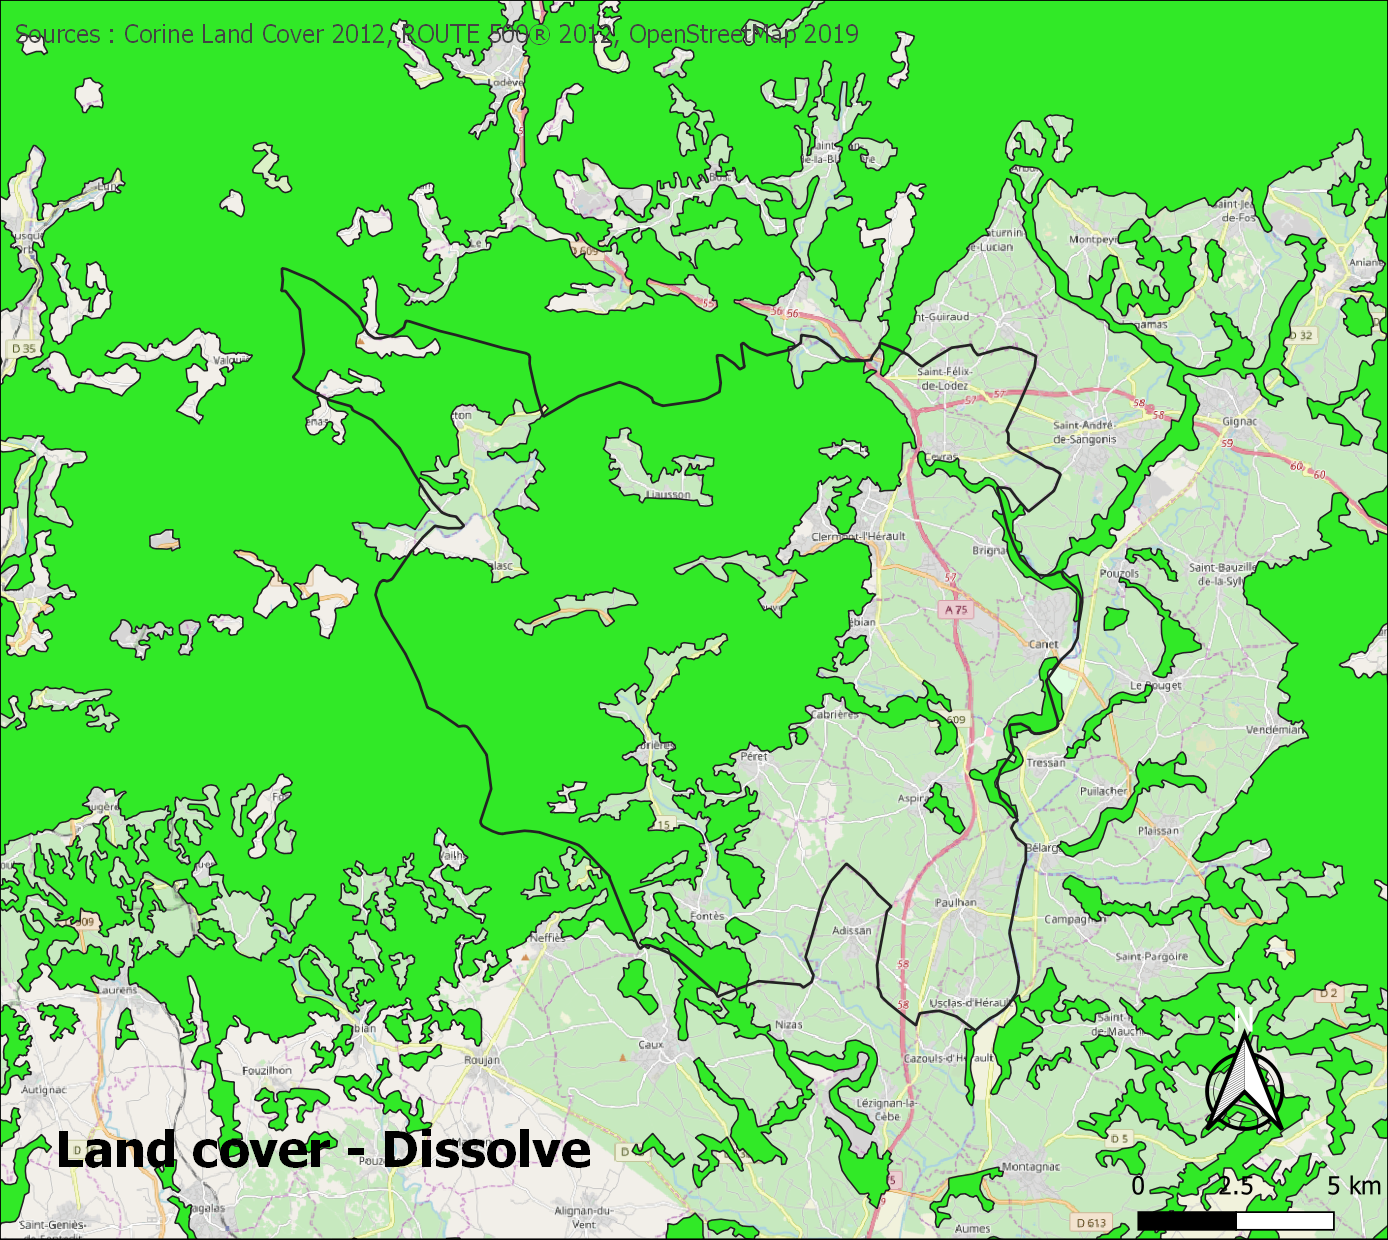
\includegraphics[width=\textwidth]{pictures/CBC/cbcLanduseDissolve.png}
      \caption{Étape 2}
   \end{subfigure}
   \begin{subfigure}[b]{.48\textwidth}
      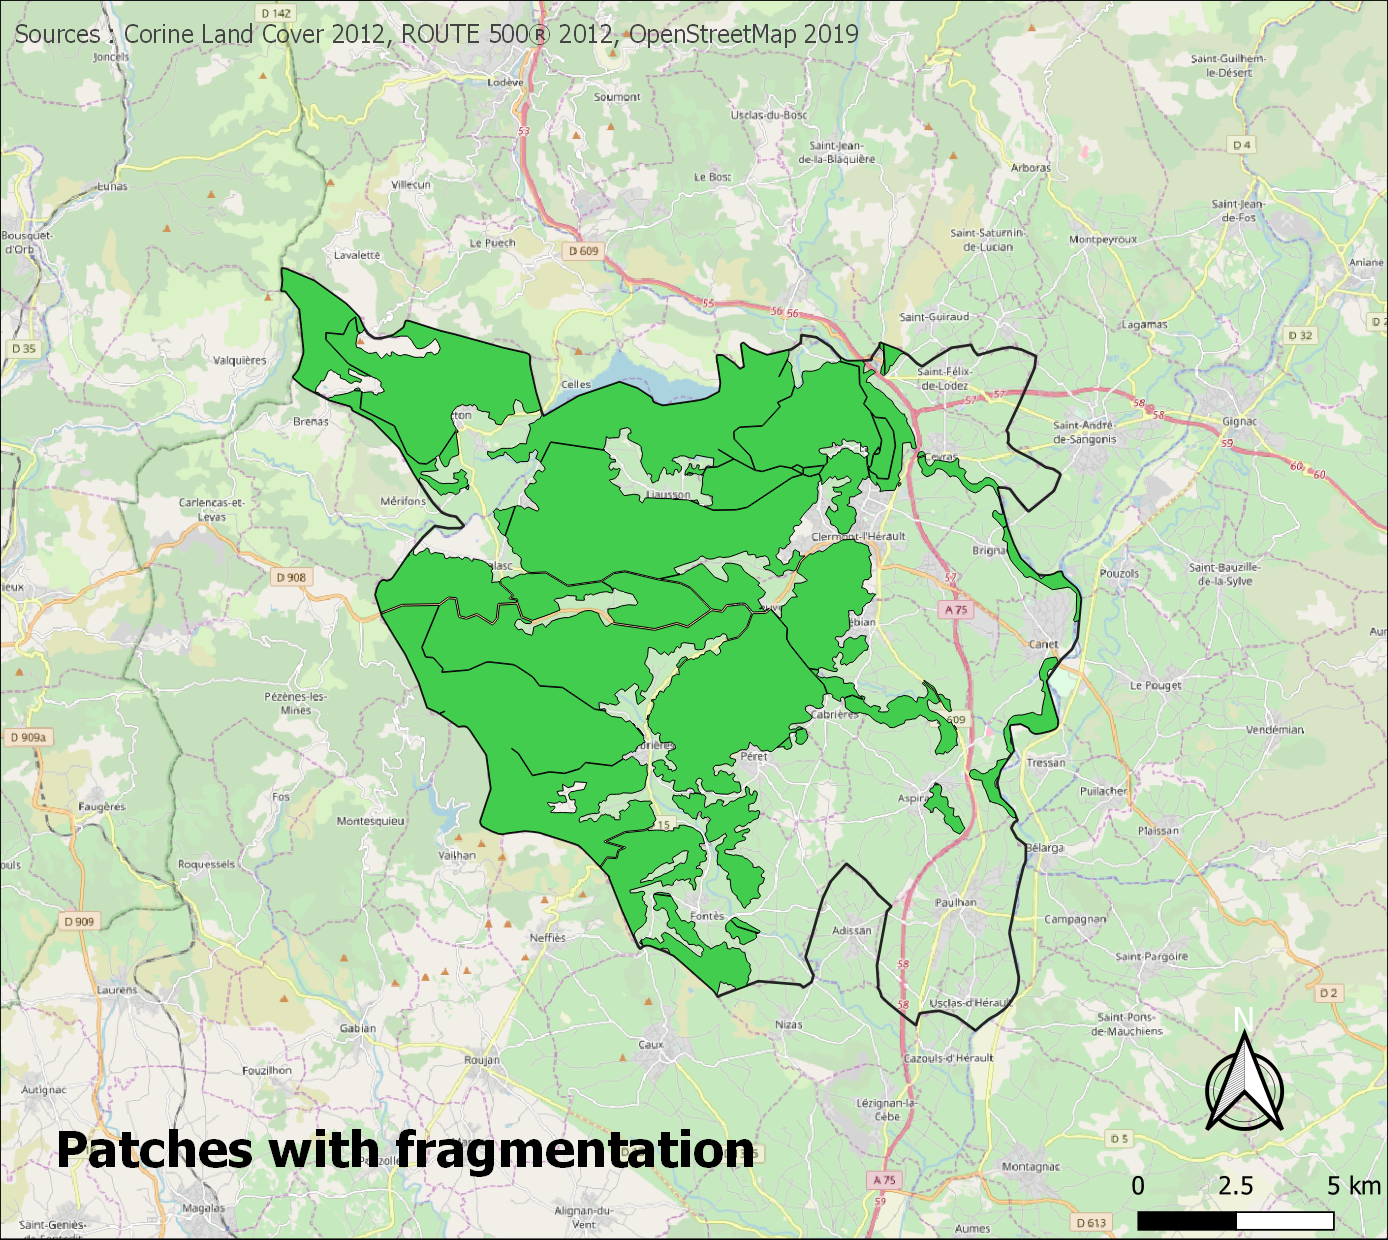
\includegraphics[width=\textwidth]{pictures/fragmPatches.png}
      %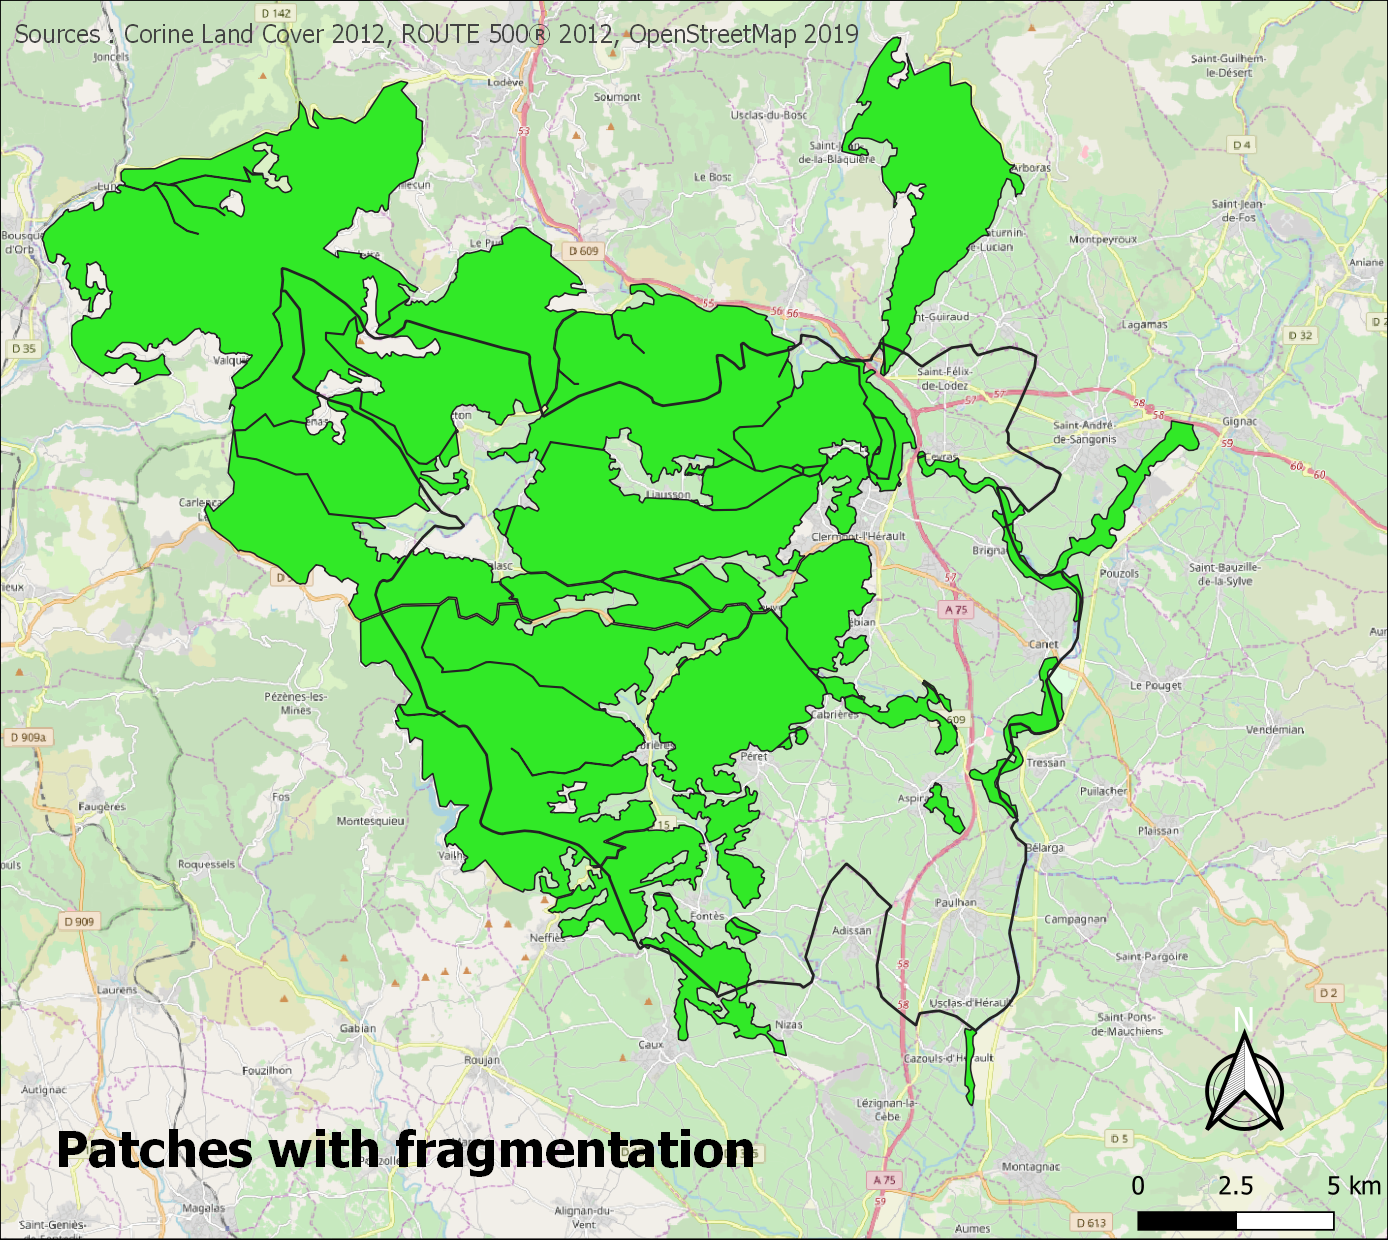
\includegraphics[width=\textwidth]{pictures/CBC/cbcFragmPatches.png}
      \caption{Étape 3}
   \end{subfigure}
   \begin{subfigure}[b]{.48\textwidth}
      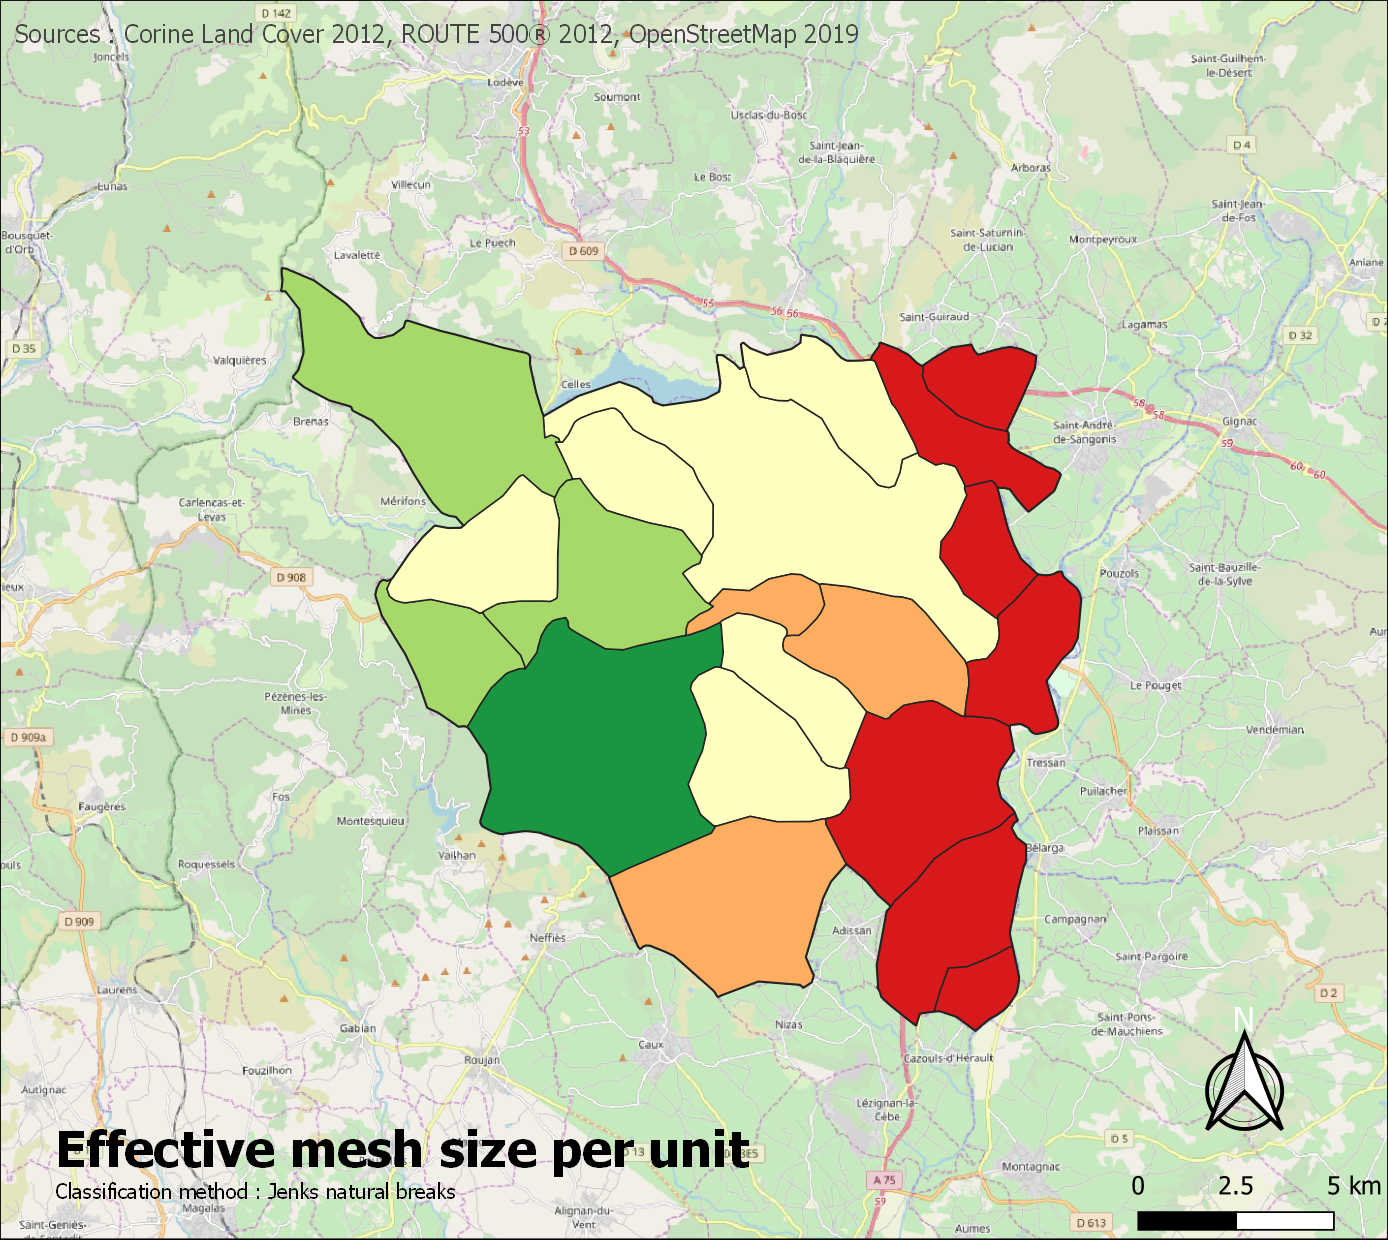
\includegraphics[width=\textwidth]{pictures/results.png}
      %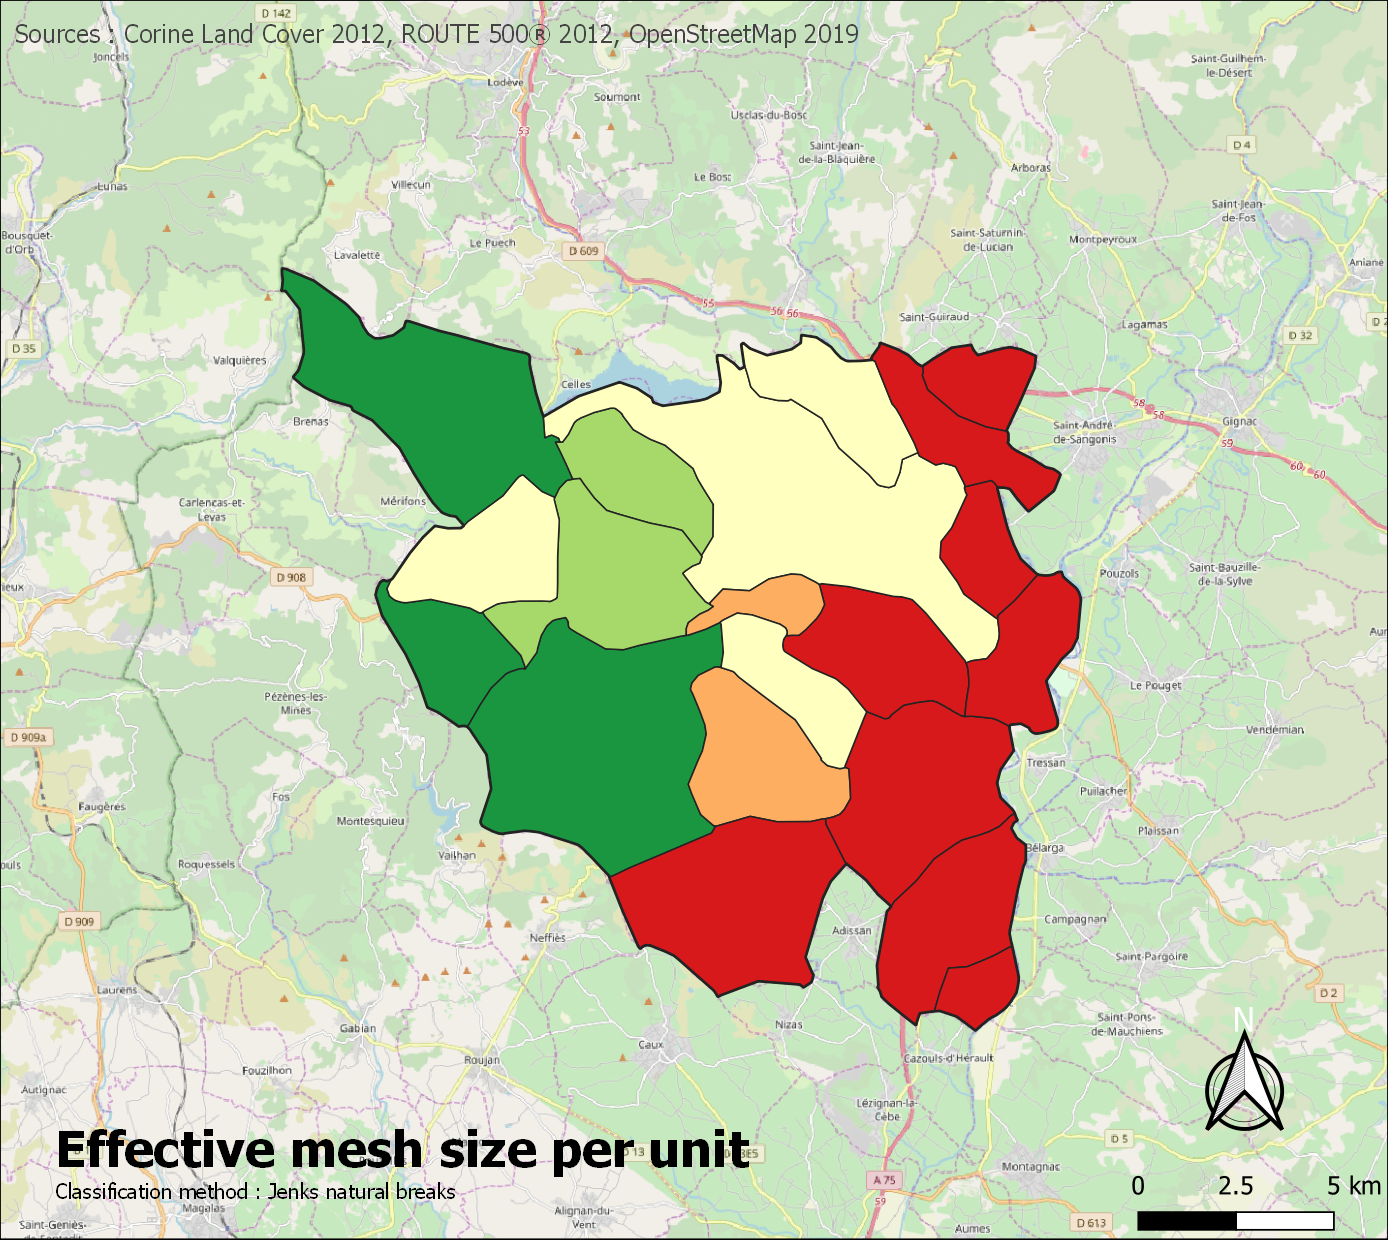
\includegraphics[width=\textwidth]{pictures/CBC/cbcResults.png}
      \caption{Étape 4}
   \end{subfigure}
   \caption{Cas d'utilisation de \tool\ : des données brutes à la taille effective de maille}
   \label{fig:usecase}
\end{figure}

La figure \ref{fig:usecase} montre l'occupation du sol initiale et le résultat de chaque étape.

Pour reproduire les résultats :
\begin{itemize}
    \item Copier le répertoire \texttt{sample\_data} localement
    \item Ouvrir \tool
    \item Choisir le dossier (\texttt{sample\_data/CUT}) comme dossier de travail
    \item Ouvrir le fichier de configuration \texttt{EPCI\_Clermontais\_2012\_CUT.xml} (icône   \includesvg[scale=0.6]{pictures/mActionFileOpen.svg})
    \item Vérifier que la configuration a été correctement chargée
    \item Lancer les étapes 2 puis 3 puis 4
\end{itemize}

%Legends are not automatically generated.



%\animategraphics[autoplay,loop,width=\textwidth,controls,scale=0.5]{1}{pictures/Image_}{1}{4}

\section{Pour aller plus loin...}



\subsection{Temps d'exécution et mémoire vive}
\label{sec:execTime}

L'utilisation de \tool\ peut être limitée par les ressources informatiques disponibles en cas d'application à de larges territoires à des niveaux de précision élevés.

\subsubsection{Mode vecteur}

En mode vecteur, le frein est le temps d'exécution du programme qui dépend de l'étendue et de la précision des données.

La figure \ref{fig:benchCLC} montre l'évolution du temps d'exécution en fonction de l'étendue de la zone d'étude (département / région / France entière) à partir de données \emph{Corine Land Cover} (format vecteur) :

\begin{figure}[h!]
\begin{center}
\begin{tabular}{|c|ccc|}
    \hline
    Cas de test & Étape 2 & Étape 3 & Étape 4\\
    \hline
    Hérault & <1mn & 1mn & 1mn \\
    Occitanie & 5mn & 11mn & 2mn \\
    France & 122h & 19h & 5h \\
    \hline
\end{tabular}
\end{center}
\vspace*{-0.5cm}
\caption{Temps d'exécution en fonction de l'étendue}
\label{fig:benchCLC}
\end{figure}

La figure \ref{fig:benchOS} montre la différence de temps de traitement entre 2 sources de données (\emph{Corine Land Cover} et \emph{OCcupation du Sol Grande Échelle}) pour un même territoire (département de l'Hérault) :

\begin{figure}[h!]
\begin{center}
\begin{tabular}{|c|ccc|}
    \hline
    Cas de test & Étape 2 & Étape 3 & Étape 4\\
    \hline
    CLC & <1mn & 1mn & 1mn \\
    OCSGE & 6h & 35h & 3mn \\
    \hline
\end{tabular}
\end{center}
\vspace*{-0.5cm}
\caption{Temps d'exécution - CLC vs OCSGE}
\label{fig:benchOS}
\end{figure}

Si le temps d'exécution est trop grand, une possibilité est de passer en mode raster. Cela permet de garder la précision typologique de la source de données au prix d'une dégradation de la précision géométrique (dégradation faible à de petites résolutions).

\subsubsection{Mode raster}

En mode raster, la ressource plus critique est la mémoire vive (RAM) qui dépend de la taille des données traitées (le nombre de pixels). Le volume de données est directement lié au couple \texttt{(étendue,  résolution)}, ainsi s'il manque de la mémoire vive il est conseillé de dégrader (augmenter) la résolution.

\end{center}

%\subsection{Algorithms}

\subsection{Algorithmes}
\label{sec:algs}

Les algorithmes (disponibles dans la boîte à outils de traitements de \qgis) implémentent la plupart des traitements spécifiques de \tool. La figure \ref{fig:algs} montre les algorithmes disponibles. Les groupes \texttt{Raster} et \texttt{Vector} correspondent à des étapes décrites en section \ref{sec:steps}.

\begin{minipage}[c]{.46\linewidth}
\begin{enumerate}
    \item \texttt{Compare results layer} : calcul de la différence entre 2 couches résultats de \tool\ pour chaque champ (cf section \ref{sec:cmp})
    \item \texttt{Raster Effective Mesh Size} : calcul des indicateurs de fragmentation en mode raster sans couche de rapportage
    \item \texttt{Raster Effective Mesh Size (Cross-Boundary Connection)} : calcul des indicateurs de fragmentation en mode raster et CBC
    \item \texttt{Raster Effective Mesh Size per feature} : calcul des indicateurs de fragmentation en mode raster selon une couche de rapportage
\end{enumerate}
\end{minipage} \hfill
\begin{minipage}[c]{.5\linewidth}
    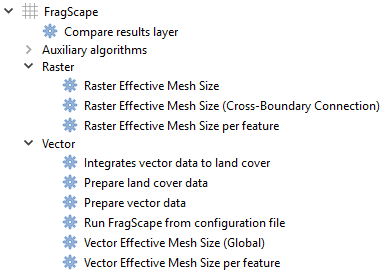
\includegraphics[scale=1]{pictures/algs_v2.png}
    \captionof{figure}{Algorithmes de \tool}
    \label{fig:algs}
\end{minipage}

\begin{enumerate}
    \item \texttt{Integrates vector data to land cover} : application de la différence/union (géométrique) entre la couche d'espaces naturels avec les données complémentaires en mode vecteur
    \item \texttt{Prepare land cover data} : sélection des espaces naturels depuis l'occupation du sol en mode vecteur
    \item \texttt{Vector Effective Mesh Size (Global)} :  calcul des indicateurs de fragmentation en mode vecteur sur l'ensemble du territoire (les entités sont fusionnées si nécessaire)
    \item \texttt{Vector Effective Mesh Size per feature} :  calcul des indicateurs de fragmentation en mode vecteur pour chaque entité de la couche de rapportage
\end{enumerate}


\subsection{Comparaison de résultats}

L'objectif de \tool\ est d'étudier l'évolution de la fragmentation et donc de comparer les résultats entre eux. L'algorithme \texttt{Compare results layer} permet de calculer l'évolution de chaque métrique de fragmentation. Il est possible de comparer des unités territoriales de même échelle (le résultat dépendant de la surface) mais l'indicateur de taille effective de maille a été conçu pour comparer la fragmentation d'un même territoire à 2 dates différentes.

Pour la différence sur les champs \texttt{effective\_mesh\_size} et \texttt{net\_product}, la valeur en mode CBC est retenue si elle existe.

Le champ \texttt{variation} contient le pourcentage d'évolution de la taille effective de maille : $(B_{val} - A_{val} ) / (B_{val} + A_{val})$.

\subsection{Sensibilité}
\label{sec:cmp}

Les résultats sont très sensibles au paramétrage de l'outil. Plusieurs critères peuvent expliquer cette sensibilité :
\begin{itemize}
    \item la sélection des espaces naturels peut varier selon les sources de données
    \item la sélection des éléments fragmentants : \textbf{critère le plus important}
    \item la taille des zones tampons (peu d'impact entre faibles valeurs puis impact exponentiel)
    \item la résolution en mode raster (peu d'impact entre faibles valeurs puis impact exponentiel)
\end{itemize}

Pour pouvoir étudier l'évolution de la fragmentation il faut donc que ces critères soient stables, c'est-à-dire :
\begin{itemize}
    \item choisir une couche d'occupation du sol produite avec une méthode et une typologie stable (éviter les changements de nomenclature par exemple)
    \item choisir un critère de sélection stalbe pour les éléments de fragmentantes (par exemple se baser sur la classe administrative d'une route est déconseillée car une route peut être déclassée, ce qui mènerait à une perte de fragmentation artificielle)
    \item garder les mêmes paramètres (taille de tampon, résolution, couche d'étude, ...)
\end{itemize}

\subsection{Fichier de configuration}

La configuration est enregistrée dans un fichier XML et peut donc être ouverte dans un éditeur de texte. La figure \ref{fig:configFile} détaille le contenu du fichier de configuration \texttt{sample\_data/ECPI\_Clermontais\_2012/CBC/ECPI\_Clermontais\_2012\_CBC.xml}

\begin{figure}[h!]
    \centering
    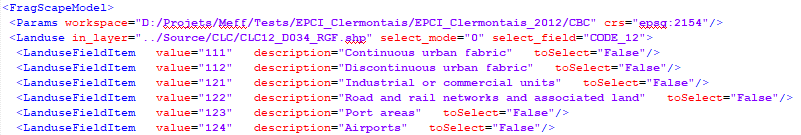
\includegraphics[scale=0.8]{pictures/configFile.png}
    \caption{Exemple de fichier de configuration}
    \label{fig:configFile}
    %\source{\tool\ v1.0}
\end{figure}

La balise \textit{Landuse} correspond à l'étape 2 et contient les attributs \textit{in\_layer} (couche d'entrée), \textit{select\_mode} ($0$ correspondant au mode de sélection \texttt{Par valeur de champ}) et \textit{select\_field} (champ de sélection de la couche d'entrée, ici \textit{CODE\_12}).
Pour chaque valeur de champ chargée, il existe une balise \textit{LanduseFieldItem} contenant les mêmes attributs que dans \tool\ (\textit{value}, \textit{description}, \textit{toSelect}).

Le fichier de configuration peut être édité manuellement si besoin, par exemple si les chemins relatifs doivent être adaptés à une nouvelle hiérarchie de fichier (\texttt{../Source} devenant \texttt{../../Source}). Éditer manuellement le fichier et le recharger dans \tool\ est alors plus simple que de changer les valeurs dans l'interface graphique.


\section{FAQ}

\begin{itemize}
\item \textbf{Les champs ne sont pas chargés dans le widget \includesvg{pictures/mIconExpression.svg}, pourquoi ?} Si les champs n'apparaissent pas, c'est que la couche associée n'a pas été chargée même si elle apparaît dans la liste déroulante. Sélectionner une autre couche puis re-sélectionner la couche initiale.

\item \textbf{Quelle méthode dois-je utiliser, CUT ou CBC ?} La méthode CBC a été conçue pour répondre au biais dû à l'«effet frontière» et il est donc conseillé de l'utiliser. La méthode CUT est disponible pour permettre la comparaison avec d'ancien résultats ou si les frontières ne sont pas problématiques.

\item \textbf{Les éléments de fragmentation sont déjà inclus dans la couche d'occupation du sol, dois-je lancer l'étape 3 quand même ?} Dans \tool\ 2.0, il est possible de spécifier la couche d'entrée de l'étape 4 et donc de ne pas lancer l'étape 3.

\item \textbf{Puis-je appliquer les traitements de \tool\ à une couche non produite par \tool\ ?} Pour appliquer un traitement spécifique de \tool\ à des données spécifiques, il est possible d'utiliser les algorithmes de \tool\ décrits en section \ref{sec:algs}.

\end{itemize}

\frameboxbegin{Bonnes pratiques}
\begin{itemize}
    \item Ne pas utiliser d'espaces ni de caractères spéciaux dans les noms de fichier.
    \item Ne pas utiliser de caractères spéciaux ni d'accents dans les valeurs de champ.
    \item Sauvegarder la configuration de \tool\ régulièrement.
    \item Vérifier le résultats de chaque étape.
    \item Si un bug inexpliqué survient, sauvegarder la configuration, quitter \tool\, relancer \tool\ et recharger la configuration sauvegardée. Si le bug persiste, quitter et relancer QGIS. Si le bug persiste toujours, contacter l'équipe de support.
\end{itemize}
\frameboxend

\subsection{Messages d'erreur}
\label{sec:err}

\begin{itemize}
    \item \textbf{\color{red}Layer XXX is already loaded in QGIS, please remove it.} \tool\ ne peut pas supprimer un fichier s'il est déjà chargé dans QGIS. Supprimer la couche XXX de QGIS et relancer le traitement \tool.
    \item \textbf{\color{red}The process cannot access the file because it is being used by another process: XXX.} Vérifier que le fichier XXX n'est pas utilisé par un autre programme ou, s'il vient d'être utilisé dans \qgis, attendre un peu et relander le traitement. Si ce n'est pas le cas, quitter et relancer QGIS, relancer \tool, réouvrir le fichier de configuration et relancer le traitement \tool.  
    \item \textbf{\color{red}Algorithm XXX not found} Cette erreur arrive si \tool\ a mal été installé. Pour y rémédier, désinstaller puis résintaller le plugin. Si l'erreur persiste, contacter l'équipe du support.
    %\item \textbf{\color{red}ModuleNotFoundError: No module named 'scipy'|'numpy}
    \item \textbf{\color{red}NameError: name 'np'|'scipy' is not defined}
    La bibliothèque \emph{scipy}|\emph{numpy} n'est pas installée. Il faut l'installer et relancer \qgis. Sous \emph{Linux}, installer le paquet \emph{python-scipy}|\emph{python-numpy}. Sous \emph{Windows}, utiliser l'installeur \emph{OsGeo4W}.
}
\end{itemize}

Si un message d'erreur inconnu apparaît, créer un nouveau ticket à l'adresse \url{https://github.com/MathieuChailloux/FragScape/issues}.

%\subsubsection*{}

\addcontentsline{toc}{section}{Bibliographie}
\printbibliography

\end{document}